% A Tex File using this template for reference
% Author: LiPtP

\documentclass{SEU-AI-Report}

\setstudentinfo{61522529}{李勃璘}{2025}{3}{25}

\begin{document}

\title{1}{支持向量机}

\section{实验目的}
了解支持向量机(Supported Vector Machine, SVM)的基本概念及原理,了解核函
数的基本原理以及作用。通过实验学会 SVM 在简单分类问题中的应用并通过
SVM构建一个垃圾邮件分类系统。

\section{实验内容}
本实验使用Python语言(Python 3.10.6)完成,依赖的第三方库包括Sklearn(一个强力的机器学习库)、Scipy(用于数学处理的软件包)、Numpy(一种开源的数值计算扩展库)以及nltk(自然语言处理工具包)。

本实验使用的数据集如表~\ref{tab:dataset}~所示。在SVM训练的实验中主要使用前三个训练集,而对于垃圾邮件分类,则需要训练集、测试集以及垃圾邮件与正常文件的样本。多维样本以\texttt{.mat}格式给出,文本格式的样本以\texttt{.txt}格式给出。
\begin{table}[htbp]
    \centering
    
    
    \begin{tabular}{cc}
        \toprule
        数据集 & 意义 \\
        \midrule
        dataset\_1.mat		& 线性可分SVM数据集\\
        dataset\_2.mat		& 非线性可分SVM数据集\\
        dataset\_3.mat		& 非线性可分SVM数据集\\
        spamTrain.mat		& 垃圾邮件训练集\\
        spamTest.mat		& 垃圾邮件测试集\\
        vocab.txt			& 词典映射文件\\
        emailSample1.txt	& 邮件样本1\\
        emailSample2.txt	& 邮件样本2\\
        spamSample1.txt		& 垃圾邮件样本1\\
        spamSample2.txt		& 垃圾邮件样本2\\
        \bottomrule

    \end{tabular}
    \caption{实验使用数据集}
    \label{tab:dataset}
\end{table}
\subsection{线性可分SVM}

\CodeReference{附录~\ref{sec:SVM}~的part1函数}



首先使用\texttt{scipy}库导入\texttt{.mat}类型的线性可分数据集1,并使用\texttt{matplotlib}库绘图。绘图的结果如图~\ref{fig:dataset1}~所示。

\begin{figure}[htbp]
    \centering
    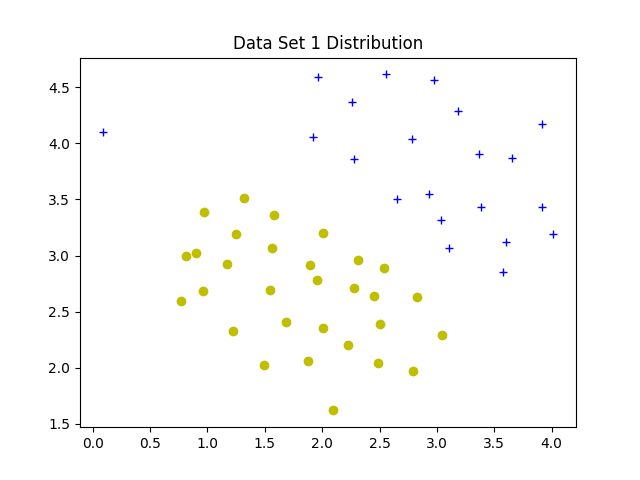
\includegraphics[width=0.5\textwidth]{figure/fig1.png}
    \caption{数据集 1(线性可分)可视化}
    \label{fig:dataset1}
\end{figure}
\figureAnalyze{显然可以看到两种类型的数据大体可以通过线性决策边界分开,但有少量用于测试模型性能的离群点。因此可称这种数据集为线性可分数据集。}

分别调用$C = 1$和$C = 100$ 下的绘制SVM决策边界函数(\texttt{visualize\_boundary}),得到不同$C$参数下数据集1的SVM决策边界如图~\ref{fig:result1}。可以看到,$C=100$时的决策边界包含了蓝色离群点,这是因为$C=100$时模型错误分类的惩罚权重更大,因此模型更倾向于包含离群点。
\begin{figure}[htbp]
    \centering
    \subfloat[$C=1$]{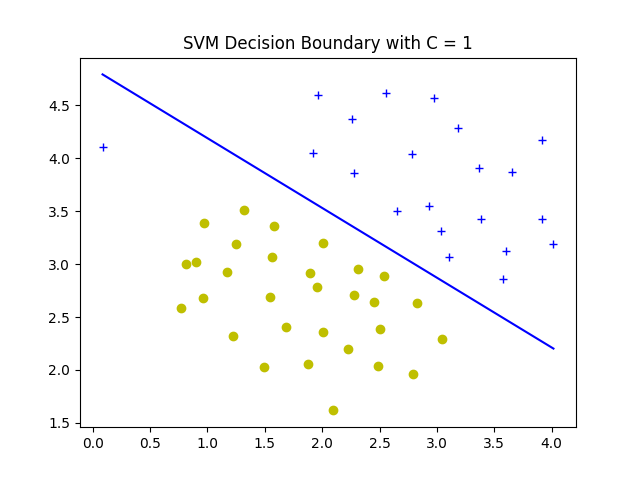
\includegraphics[width=0.45\textwidth]{figure/fig2.png}}
    \hfill
    \subfloat[$C=100$]{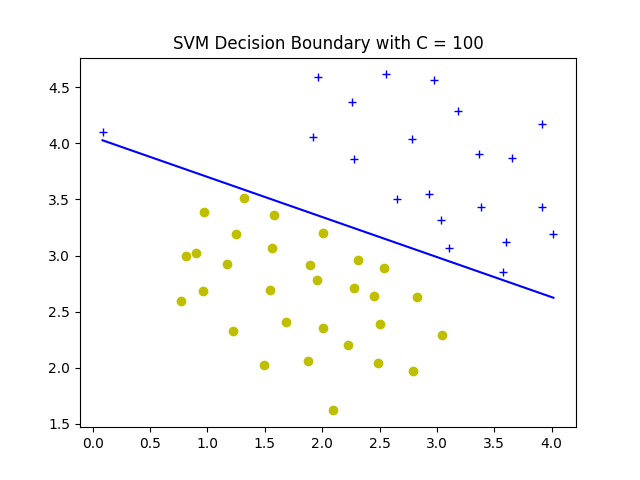
\includegraphics[width=0.45\textwidth]{figure/fig3.png}}
    \caption{不同$C$参数下数据集1的SVM决策边界}
    \label{fig:result1}
\end{figure}

\subsection{非线性可分SVM}
\CodeReference{附录~\ref{sec:SVM}~的part2函数}

线性不可分指的是无法通过一个线性决策面来完美分隔数据集,这时候会出现分类错误。尽管线性可分的数据集分类方式简单,但这种数据集不具备普遍性。因此,需要找到一种方法处理非线性可分的数据集。

为了处理非线性可分的数据集,需要引入高斯核。它在SVM中也被称为径向基核函数(Radial Basis Function, RBF),定义如下:
\begin{equation}
K(x_i, x_j) = \exp\left(-\gamma \|x_i - x_j\|^2\right)
\end{equation}
其中,$\gamma$ 是一个超参数,控制高斯核的影响范围。较大的 $\gamma$ 使得模型更加关注局部信息,而较小的 $\gamma$ 使得模型能够捕捉全局结构。

为了测试高斯核函数,使用它计算两个一维样本\texttt{[1,2,1]}和\texttt{[0,4,-1]}的相似度。这段代码的输出结果为:Similarity between object 1 and object 2: 0.324652。(\CodeReference{附录~\ref{sec:SVM}~的part2函数,gaussian\_kernel函数})结果验证正确。

接下来训练非线性SVM。首先绘制出非线性可分的数据集2如图~\ref{fig:dataset2}。可以看到正负样本间存在非线性的边界。
\begin{figure}[htbp]
    \centering
    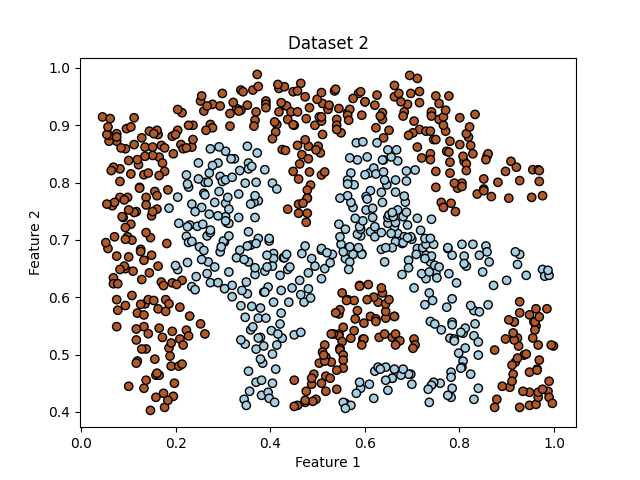
\includegraphics[width=0.5\textwidth]{figure/fig4.png}
    \caption{数据集 2(线性不可分)可视化}
    \label{fig:dataset2}
\end{figure}

使用SVM的\texttt{fit}方法训练SVM,画出拟合决策边界如图~\ref{fig:result2}。可以看到SVM基本正确地拟合了数据集2的非线性边界。

\begin{figure}[htbp]
    \centering
    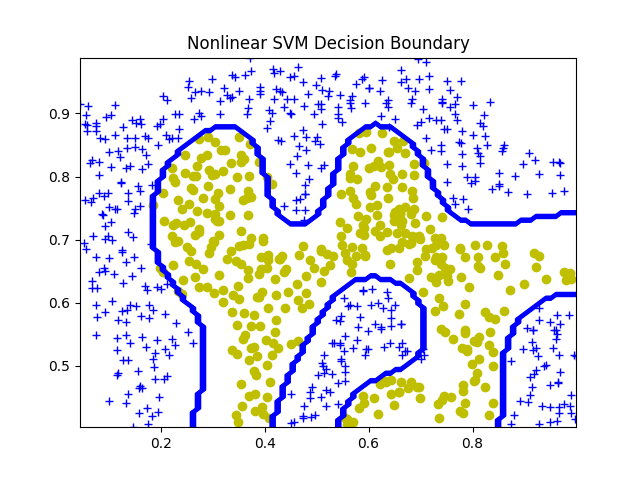
\includegraphics[width=0.5\textwidth]{figure/fig5.png}
    \caption{数据集 2的SVM决策边界}
    \label{fig:result2}
\end{figure}
实验结果表明,高斯核方法能够有效处理非线性可分的数据集,并在较为复杂的数据结构中取得良好的分类效果。此外,超参数 $\gamma$ 的选择对分类性能有重要影响,需要通过交叉验证或网格搜索进行优化。
\subsection{最优参数搜索}
\CodeReference{附录~\ref{sec:SVM}~的part3函数}

在数据集3中,数据被划分为了训练集以及验证集。绘制训练集和验证集以观察数据(图~\ref{fig:dataset3}~):
\begin{figure}[htbp]
    \centering
    \subfloat[训练集]{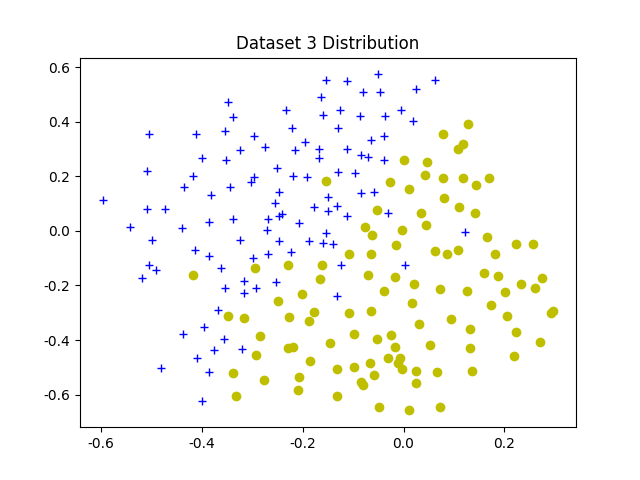
\includegraphics[width=0.45\textwidth]{figure/fig6.png}}
    \hfill
    \subfloat[验证集]{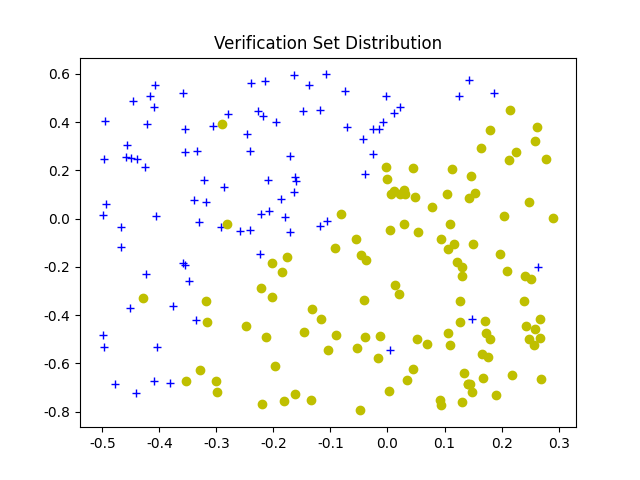
\includegraphics[width=0.45\textwidth]{figure/fig_verification.png}}
    \caption{数据集3的训练集和验证集}
    \label{fig:dataset3}
\end{figure}

基于训练集训练的模型将在验证集上进行测试并根据验证集的反馈结果对模型参数进行微调。参数$C$和$\sigma$的搜索空间为\texttt{[0.01, 0.03, 0.1, 0.3, 1, 3, 10, 30]}。确定最优参数组合后(\CodeReference{附录~\ref{sec:SVM}~的params\_search函数})训练,得到的决策边界如图~\ref{fig:result3}~所示。从图中可以看出SVM模型已经尽可能正负样本分开,但是还是存在少量样本未被彻底分开,如果要将其分开可能导致过拟合。
\begin{figure}[htbp]
    \centering
    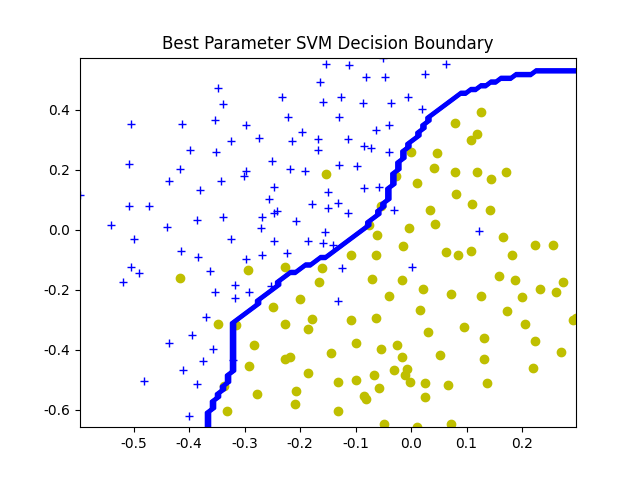
\includegraphics[width=0.5\textwidth]{figure/fig7.png}
    \caption{数据集3的决策边界}
    \label{fig:result3}
\end{figure}
\subsection{垃圾邮件分类}
\CodeReference
\section{提高训练}
基于实验手册的内容,尝试对现有实验做修改和调整,如损失函数、激活函数等。

\section{实验心得}

在本次实验中,我理解了支持向量机的基本工作流程以及使用Python训练SVM模型,拟合线性、非线性边界的基本方法。并基于SVM完成了垃圾邮件分类识别的小实验。另外,我还独立编写了\LaTeX 模板(\texttt{SEU-AI-Report.cls}),用于本实验报告的撰写。在这个过程中也学到了不少关于\LaTeX 的进阶知识。

\nocite{qiu2020nndl}
\printbibliography

\appendix
\section{实验代码}
该部分列举本实验中使用的所有实验代码。
\subsection{SVM训练相关代码}\label{sec:SVM}
\pythoncode[caption = ex3.py]{ex3.py}
\subsection{垃圾邮件分类相关代码}\label{sec:spam}
\pythoncode[caption = ex3\_spam.py]{spam.py}

\end{document}
